\chapter{Pianificazione}

Scadenze:
\begin{itemize}
    \item RTB (Requirements and Technology Baseline) : 28/02/2022;
    \item PB (Product Baseline) : 04/04/2022;
    \item CA (Customer Acceptance) : 02/05/2022.
\end{itemize}

\section{Verso la RTB}

\textit{Periodo: 29/11/2021 - 28/02/2021}

\subsection{Primo periodo}

\textit{Periodo: 29/11/2021 - 18/12/2021}

In questa prima fase risulta di priorità massima discutere tutte le regole già introdotte
e applicate nello svolgimento del progetto che però non sono ancora state documentate.
Questo per avere un documento scritto a disposizione di tutti i membri che consenta di
non avere dubbi su come svolgere qualsiasi attività e su come utilizzare le risorse.
\par In questa fase è importante anche individuare tutti i vari rischi che possono portare
problemi allo svolgimento del progetto per non essere colti di sorpresa.
\par Di fondamentale importanza è anche iniziare a pianificare le prime attività e quindi
le prime milestone in modo da organizzare le risorse e di fornire un preventivo$_G$. 

\begin{figure}[!ht]
    \includegraphics[width=1.0\textwidth]{Gantt1}
    \caption{Diagramma di Gantt della prima milestone} 
\end{figure}

\newpage

\subsection{Secondo periodo}

\textit{Periodo: 20/12/2021 - 10/01/2022}

In questa fase diventa importante analizzare nel dettaglio il capitolato per riuscire a
cogliere i casi d'uso necessari. Inoltre, per evitare dubbi e per non effettuare
scelte sbagliate, sarà opportuno organizzare uno o più incontri con il proponente in modo da
condividere idee e dubbi sorti durante l'analisi che sarà sicuramente più approfondita di quella
effettuata durante la scelta del capitolato.
\par Da tutto ciò si inizierà a redarre l'\textit{Analisi dei Requisiti}, documento importantissimo per il progetto poiché
conterrà tutti i casi d'uso individuati, i requisiti obbligatori, quelli desiderabili e quelli opzionali.
\par In questa fase è opportuno stilare anche il \textit{Piano di Qualifica}, necessario per individuare
i metodi per garantire la qualità di processo e di prodotto.

\begin{figure}[!ht]
    \includegraphics[width=1.0\textwidth]{Gantt2}
    \caption{Diagramma di Gantt della seconda milestone} 
\end{figure}

\subsection{Terzo periodo}

\textit{Periodo: 15/01/2022 - 04/02/2022}

Dopo avere avuto un colloquio con il proponente sui casi d'uso e i requisiti è importante progredire con
l'\textit{Analisi dei Requisiti}. Diventa, poi, fondamentale studiare le tecnologie e gli strumenti necessari
per realizzare il prodotto. Questo permetterà di realizzare il PoC (Proof of Concept)$_G$, una versione semplificata 
del prodotto finale che permetta di intuire se la direzione è quella giusta e che mostri al proponente se lo 
sviluppo è corretto.

\begin{figure}[!ht]
    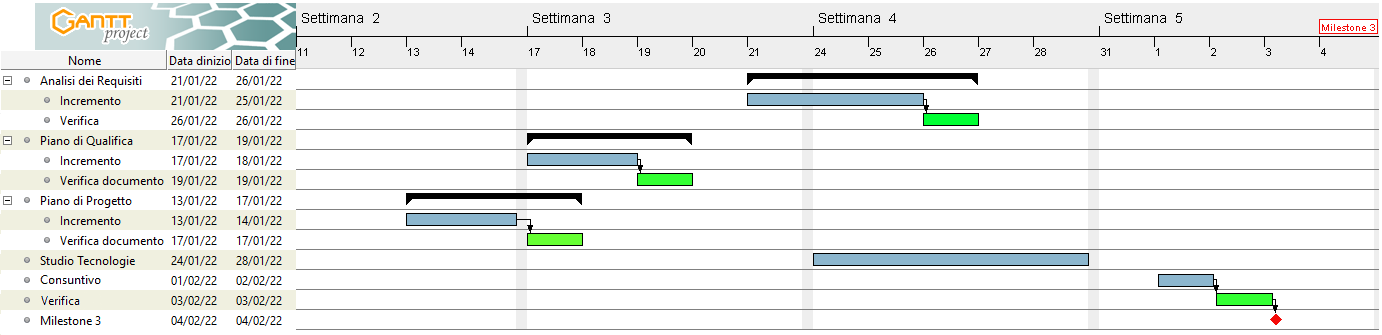
\includegraphics[width=1.0\textwidth]{Gantt3.png}
    \caption{Diagramma di Gantt della terza milestone} 
\end{figure}


\subsection{Quarto periodo}
\textit{Periodo: 7/02/2022 - 24/02/2022}

In quest'ultimo periodo diventa di fondamentale importanza la progettazione e la realizzazione
 del PoC. Inoltre diviene necessario il completamento e la verifica finale dei documenti prima della revisione prevista 
 per fine febbraio.


\begin{figure}[!ht]
    \includegraphics[width=1.0\textwidth]{Gantt4.png}
    \caption{Diagramma di Gantt della quarta milestone} 
\end{figure}

\section{Verso la PB}

\textit{Periodo: 29/02/2022 - 04/04/2022}

Superata la prima revisione, l'obiettivo principale è realizzare una prima versione del prodotto finale che dimostri come ha già fatto il PoC, nella sua semplicità, 
che requisiti e tecnologie scelte possono coesistere nello stesso prodotto. 

Sarà, quindi, fondamentale la progettazione per arrivare ad avere un design$_G$ che sia quello definitivo e poi avere un avanzamento consistente di codifica e verifica.

Viste le difficoltà riscontrate nella pianificazione a lungo termine, preferiamo aspettare di superare la revisione precedente per poi poterci dedicare nel dettaglio
alla pianificazione dei periodi che caratterizzeranno l'intera milestone.

\section{Verso la CA}

\textit{Periodo: 05/04/2022 - 02/05/2022}

Superata la seconda revisione, l'obiettivo rimane quello di presentare al proponente il prodotto finale.

Sarà quindi necessario adattare il prodotto realizzato ai feedback$_G$ ricevuti nella revisione precedente e fare in modo che il prodotto superi tutti i test. Inoltre, bisognerà
verificare che il prodotto rispecchi le richieste del proponente poichè dovrà superare un vero e proprio collaudo.

Anche in questo caso, la pianificazione nel dettaglio sarà fatta in un secondo momento più opportuno e in condizioni migliori.